% Course report for the FiDIP hands-on exercise, EECE 7373.
% Build in this folder: tectonic report.tex
% Figures: python scripts/make_report_figures.py writes results/figures/.
\documentclass[11pt]{article}
\usepackage[margin=1in]{geometry}
\usepackage[T1]{fontenc}
\usepackage{lmodern}
\usepackage{microtype}
\usepackage{graphicx}
\usepackage{booktabs}
\usepackage{array}
\usepackage{enumitem}
\usepackage[font=small,labelfont=bf]{caption}
\captionsetup[table]{position=bottom}
\usepackage[numbers,sort&compress]{natbib}
\usepackage[hidelinks]{hyperref}

\graphicspath{{../results/figures/}}
\setlist{itemsep=1pt,topsep=3pt}
\setlist[enumerate]{itemsep=0pt}
\setlength{\emergencystretch}{2em}
\setlength{\intextsep}{8pt plus 2pt minus 2pt}
\setlength{\textfloatsep}{10pt plus 2pt minus 2pt}
% Let pages hold more float area, so no page ends half empty.
\renewcommand{\topfraction}{0.9}
\renewcommand{\bottomfraction}{0.8}
\renewcommand{\textfraction}{0.1}
\renewcommand{\floatpagefraction}{0.8}
\newcommand{\code}[1]{\texttt{#1}}

\title{Reproducing FiDIP Infant Pose Estimation on SyRIP}
\author{Oliver Fritsche\\EECE 7373, FiDIP hands-on exercise, Northeastern University}
\date{November 2026}

\begin{document}
\maketitle

\begin{abstract}
We reproduce FiDIP~\cite{huang2021fidip}, a pose estimator for infants, on the 100 real test images of SyRIP (Test100).
Every reported number comes from NVIDIA H200 GPUs, with the upstream code unchanged.
Our evaluation of the released checkpoint gives 93.60 AP, equal to the paper's 93.6.
This needs \code{test11.jpg} from the 2023 archive, not from the 2024 archive.
Our own training falls short.
The two upstream configs give 91.50 and 90.43 AP, against the paper's 92.7 and 93.6.
With the paper's training settings, we get 91.81 AP, still 1.8 AP below 93.6.
Five training changes do not close the gap: the best final-epoch mean is 91.88 AP.
The released checkpoint and our best reproduction run miss mostly the same joints: hidden or folded limbs.
\end{abstract}

\section{Introduction}

Pose estimators trained on adults do poorly on infants, and few labeled infant images exist.
FiDIP~\cite{huang2021fidip} adapts an adult pose model to infants with synthetic and real infant images.
The paper reports 93.6 AP on Test100.
We reproduce this number in two ways: we evaluate the released checkpoint, and we train the model ourselves.
Then we try five training changes to beat it (Section~\ref{sec:improve}).
Section~\ref{sec:repro} shows how to reproduce our results.

\section{Setup}

Table~\ref{tab:env} gives the environment, and Table~\ref{tab:data} gives the data.
Every reported number comes from one NVIDIA H200 of the cluster.
\code{scripts/check\_env.py} checks the imports, one forward pass, and the paths.
\code{scripts/prepare\_data.py} checks the image counts and sizes, and records the md5 sums of the weights.

\begin{table}[h]
\centering\small
\begin{tabular}{@{}ll@{}}
\toprule
Item & Value \\
\midrule
Compute & Explorer cluster with Slurm, one NVIDIA H200 per job \\
Software & Python 3.12, PyTorch 2.3.1, CUDA 12.1, packages in \code{requirements.txt} \\
Upstream code & FiDIP repository~\cite{fidipcode} at commit \code{a76b4f4}, unmodified \\
Our code & \code{src/}, \code{scripts/}, and \code{jobs/}; \code{MANIFEST.md} lists each job \\
Weights & Released HRNet-W48 and MobileNetV2 checkpoints, COCO DarkPose start weights \\
\bottomrule
\end{tabular}
\caption{Environment.}
\label{tab:env}
\end{table}

\begin{table}[h]
\centering\small
\begin{tabular}{@{}lrl@{}}
\toprule
Split & Images & Content \\
\midrule
Adult warm-up set & 4057 & 2029 real COCO~\cite{lin2014coco} and 2028 synthetic SURREAL~\cite{varol2017surreal} adults \\
Infant training set & 1200 & 1000 synthetic and 200 real infants \\
Test100 & 100 & Real infants: 43 supine, 41 prone, 11 sitting, 5 standing \\
\bottomrule
\end{tabular}
\caption{SyRIP splits~\cite{syrip}.}
\label{tab:data}
\end{table}

SyRIP comes in two archives: \code{SyRIP.zip} (2023) and \code{syrip\_for\_train.zip} (2024).
We use the 2024 archive, which has the layout that the upstream code reads.
In both archives, Test100 has the same images and labels, except one image.
We found two data defects:
\begin{itemize}
  \item In the 2024 archive, \code{test11.jpg} is a different photo: another scene, other clothes, another pose. Its label belongs to the photo in the 2023 archive. We use the 2023 file (Figure~\ref{fig:test11}).
  \item 46 synthetic training images are stored at 1920 by 1080, but their labels fit a 640 by 480 frame. We call them the mislabeled images. The authors trained on them, so we keep them. Section~\ref{sec:improve} tests training without them, on the cleaned data.
\end{itemize}

\section{Model and training}

FiDIP fine-tunes DarkPose~\cite{zhang2020dark}, an HRNet-W48~\cite{sun2019hrnet} with a $384\times288$ input and 17 heatmaps of $96\times72$.
A domain classifier reads the last feature map and predicts whether an image is synthetic.
Training has two stages.
First, a warm-up trains the classifier alone on the adult set.
Then the classifier and the pose network take turns.
The pose network learns to confuse the classifier, with weight \code{LAMBDA}~\cite{ganin2015dann}.
Each epoch shows 2000 infant images, half real and half synthetic, with random flips, rotations, scaling, and half-body crops.

Table~\ref{tab:configs} gives our three training configs.

\begin{table}[h]
\centering\small
\begin{tabular}{@{}lrrr@{}}
\toprule
Setting & Guide config & FiDIP config & Paper-settings config \\
\midrule
Epochs & 20 & 20 & 100 \\
Batch size & 20 & 18 & 64 \\
Warm-up epochs, batch & none & 10, 64 & 1, 128 \\
Learning rate & $10^{-4}$ & $10^{-3}$ & $10^{-3}$ \\
Learning rate $\times 0.1$ at epoch & 40, not reached & 40, not reached & 40 \\
\code{LAMBDA} & 0 & 0.0005 & 0.0005 \\
Paper's AP & 92.7 & 93.6 & 93.6 \\
\bottomrule
\end{tabular}
\caption{Our three training configs.
Guide config: the upstream file \code{w48\_384x288\_\allowbreak adam\_lr1e-3\_\allowbreak infant.yaml}, which the course guide uses.
Despite its file name, it sets learning rate $10^{-4}$. It turns FiDIP off, so it trains plain fine-tuning.
FiDIP config: the guide config with the five FiDIP values of the upstream file \code{w48\_384x288\_\allowbreak adam\_lr1e-3\_\allowbreak custom.yaml}.
Paper-settings config: the FiDIP config with the training values of the paper (Section V-B).
The paper states no learning-rate schedule, so each config keeps the drop at epoch 40 of the guide config file.}
\label{tab:configs}
\end{table}

\textbf{Implementation choices.}
\begin{itemize}
  \item We do not change the upstream code. Our scripts run its training and test code as the authors wrote it.
  \item Each training run starts from the DarkPose weights trained on adult COCO images, as the upstream README says.
  \item Each config gets three runs. The upstream trainer sets no seed, so one config gives a different AP each time.
  \item The number of a run is its final epoch. Upstream saves the best epoch by Test100 AP, which tunes on the test set. We show that number only for comparison.
\end{itemize}

\section{Evaluation}

\code{scripts/test\_model.py} runs the upstream test script on Test100.
It uses the ground-truth person boxes, the flip test, and DARK decoding.
The flip test also predicts on the mirror image, flips those heatmaps back with left and right swapped, and averages.
DARK~\cite{zhang2020dark} decodes each joint position from its heatmap to sub-pixel accuracy.
\code{pycocotools} computes the COCO keypoint AP and AR, the average recall.
Every Test100 number uses the \code{test11.jpg} of the 2023 archive, unless a table row says otherwise.
AP rests on OKS, a score from 0 to 1.
Each labeled joint gets an OKS term from 0 to 1, which falls with the distance to its label.
The distance is scaled by the person's size. OKS is the mean of the terms of a person.
AP counts a person as found when its OKS passes a threshold.
It averages over ten thresholds, from 0.50 to 0.95 in steps of 0.05. AP50 and AP75 use one threshold each.
For the analysis, we also use the OKS of each image and the OKS term of each joint.
We call a joint with an OKS term below 0.5 a missed joint.
\code{scripts/demo.py} runs the model on one image end to end.
One job, \code{jobs/reproduce\_baseline.sbatch}, runs the environment check, the evaluations of Table~\ref{tab:released}, and the demo.

\section{Results}

\begin{table}[h]
\centering\small
\begin{tabular}{@{}llrrrr@{}}
\toprule
Model & Source & AP & AP50 & AP75 & AR \\
\midrule
HRNet-W48 & Paper & 93.6 & 98.5 & 98.5 & 94.6 \\
 & Our evaluation, 2023 archive & \textbf{93.60} & 98.52 & 98.52 & 94.60 \\
 & Our evaluation, 2024 archive (Figure~\ref{fig:test11}) & 92.15 & 97.06 & 97.06 & 93.60 \\
\midrule
MobileNetV2 & Paper & 79.2 & 99.0 & 89.4 & 84.1 \\
 & Our evaluation, 2023 archive & 79.18 & 98.98 & 89.35 & 84.10 \\
\bottomrule
\end{tabular}
\caption{The released checkpoints on Test100. The archive is the source of \code{test11.jpg}.}
\label{tab:released}
\end{table}

\begin{figure}[h]
\centering
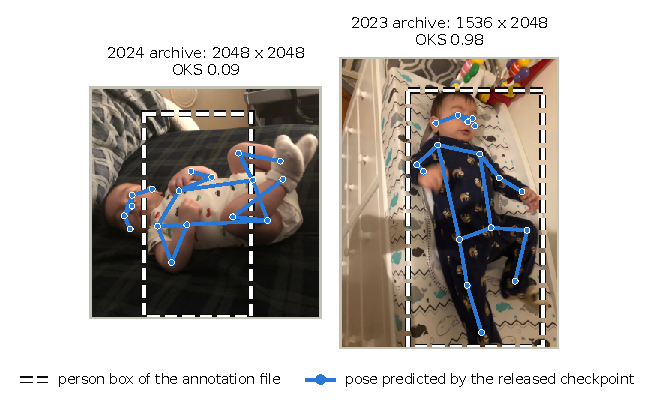
\includegraphics[width=0.52\linewidth]{test11.pdf}
\caption{\code{test11.jpg} in the two SyRIP archives. Dashed box: the person box of the annotation file. The evaluation crops a region around this box, 1.25 times larger, and the model sees only that region. Blue: the pose that the released checkpoint predicts. The 2024 file is a different photo with the label of the 2023 photo, so it scores OKS 0.09.}
\label{fig:test11}
\end{figure}

\textbf{Our evaluation of the released checkpoints matches the paper.}
The HRNet checkpoint matches all four numbers in the paper (Table~\ref{tab:released}).
With the \code{test11.jpg} of the 2024 archive, that one image scores OKS 0.09.
The AP then falls to 92.15 (Figure~\ref{fig:test11}).
The released MobileNetV2 checkpoint matches too.
So the data, the weights, and the evaluation pipeline are correct.

\begin{table}[!htb]
\centering\small
\begin{tabular}{@{}llrrrrr@{}}
\toprule
Config & Source & AP & SD & AP50 & AP75 & AR \\
\midrule
Guide config & Paper & 92.7 & & & & \\
 & Our runs & 91.50 & 0.57 & 97.75 & 97.09 & 92.67 \\
\midrule
FiDIP config & Paper & 93.6 & & & & \\
 & Our runs & 90.43 & 1.25 & 98.43 & 96.92 & 92.47 \\
\midrule
Paper-settings config & Paper & 93.6 & & & & \\
 & Our runs & \textbf{91.81} & 0.53 & 98.38 & 97.48 & 93.40 \\
\bottomrule
\end{tabular}
\caption{Our training runs on Test100: the final epoch, mean of three runs. SD: the standard deviation of the AP over the three runs. The paper reports AP only.}
\label{tab:train}
\end{table}

\begin{figure}[!htb]
\centering
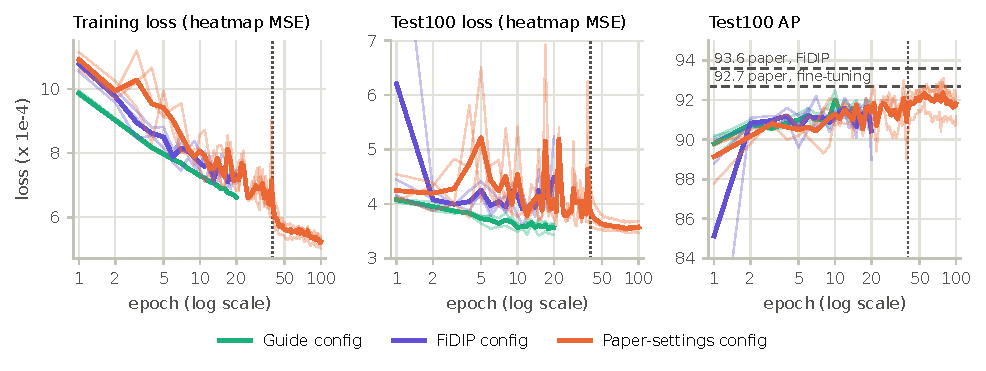
\includegraphics[width=\linewidth]{training_curves.pdf}
\caption{Per epoch, three runs per config (thin) and their mean (thick). Left: training loss. Middle: Test100 loss. Right: Test100 AP, with the paper's numbers dashed. The epoch axis is logarithmic, so the 20-epoch curves stay readable next to the 100-epoch curves. The dotted line marks the learning-rate drop of the paper-settings config at epoch 40. Loss: the mean squared error (MSE) of the heatmaps. The trainer logs the Test100 values; we never use them to choose the reported epoch.}
\label{fig:curves}
\end{figure}

\textbf{Our training falls short of the paper.}
The guide config falls 1.2 AP short, and the FiDIP config falls 3.2 AP short (Table~\ref{tab:train}).
The upstream configs train for 20 epochs instead of 100, with smaller batches (Table~\ref{tab:configs}).
The paper's settings raise the FiDIP config by 1.4 AP, to 91.81.
That is still 1.8 AP below the paper, and only 0.3 AP above the guide config.
The best epoch, chosen on Test100, gives 92.69 on average and 93.14 in the best run.
The paper does not state its epoch choice, its frozen layers, or its learning-rate schedule.
These unknowns can explain the remaining gap.

\textbf{Training curves.}
Figure~\ref{fig:curves} shows the training and Test100 curves that the guide asks for.
The guide config does not overfit: its Test100 loss falls until about epoch 10 and then stays flat.
The FiDIP config overfits: after epoch 12, its Test100 loss rises while its training loss still falls.
At learning rate $10^{-3}$, its AP also swings by up to 2 AP between epochs.
The paper-settings config swings the same way until the learning rate drops at epoch 40.
Then its Test100 loss falls until about epoch 80 and stays flat: it does not overfit.
The training loss stays above the Test100 loss, because only training images get the random augmentation.

\section{Successes and failures}

\begin{figure}[h]
\centering
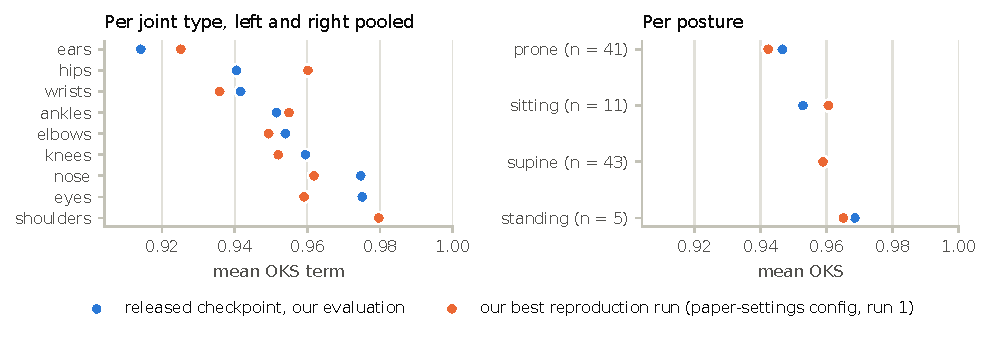
\includegraphics[width=\linewidth]{joint_posture.pdf}
\caption{Test100: our evaluation of the released checkpoint (blue) and our best reproduction run (orange). Left: mean OKS term per joint type. Right: mean OKS per posture.}
\label{fig:analysis}
\end{figure}

\begin{figure}[!htb]
\centering
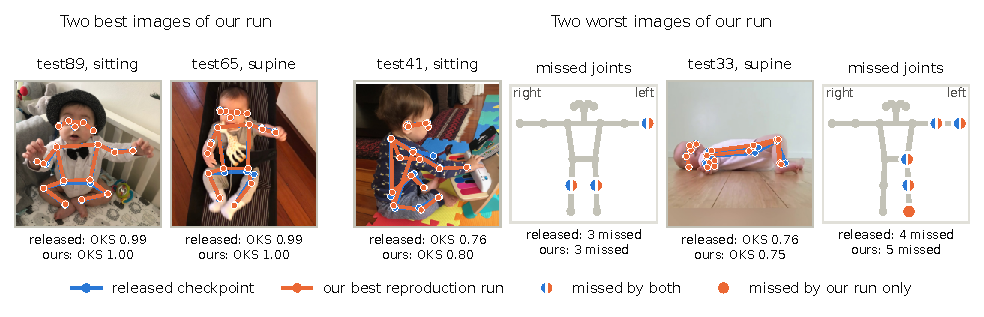
\includegraphics[width=\linewidth]{examples.pdf}
\caption{Left: the two best Test100 images of our best reproduction run, ranked by its OKS. Right: its two worst. Each photo shows our evaluation of the released checkpoint (blue) and our best reproduction run (orange). Next to each worst image, a front-facing T-pose marks the missed joints. The T-pose faces the reader, so the infant's right is on the left. A half-blue, half-orange dot marks a joint that both models miss.}
\label{fig:examples}
\end{figure}

Figures~\ref{fig:analysis} and~\ref{fig:examples} compare our evaluation of the released checkpoint with our best reproduction run.
That run is paper-settings run 1, the best of the nine runs in Table~\ref{tab:train}: 92.21 AP.
\begin{itemize}
  \item \textbf{Overall.} Our evaluation of the released checkpoint gives a mean OKS of 0.9534. 91 of 100 images score above 0.9. Our run has 0.9526 and 89 images.
  \item \textbf{Joints and postures.} Ears and wrists are among the three weakest joint types of both models. Prone is the hardest posture. The head hides one ear. A prone body hides the far limbs. Our run is better on hips and ears, but worse on eyes and nose.
  \item \textbf{Worst images.} Both models miss mostly the same joints. On \code{test41}, the legs fold under the body; both miss the left wrist and both knees. On \code{test33}, labeled supine, the infant lies on its side. Both miss the left elbow, wrist, hip, and knee. Our run also misses the left ankle.
  \item \textbf{Left and right.} Neither model mirrors a whole body. Each model swaps the two joints of only 4 of 800 left/right pairs.
\end{itemize}

\section{Improvement attempts}
\label{sec:improve}

We tried five training changes to beat the paper's number.
The changes: cleaned data, a lower learning rate, the freeze depth, a larger \code{LAMBDA}, and checkpoint choice.
Each change gets three runs with the same evaluation (Table~\ref{tab:changes}).
A sign test compares two changes image by image.
It counts the images whose mean OKS over three runs rises or falls by more than 0.01.

\begin{table}[!htb]
\centering\small
\begin{tabular}{@{}lr@{}}
\toprule
Training change & AP \\
\midrule
None: the FiDIP config & 90.43 \\
Cleaned data: no mislabeled images & 91.60 \\
Learning rate $10^{-4}$ & 91.74 \\
Both changes & 91.63 \\
Both changes, every layer trained & 91.88 \\
Both changes, stage 3 frozen too & 90.92 \\
Both changes, \code{LAMBDA} $\times 10$ & 58.55 \\
Both changes, \code{LAMBDA} $\times 100$ & 0.48 \\
\midrule
Paper (FiDIP) & 93.6 \\
\bottomrule
\end{tabular}
\caption{Training changes on Test100: final-epoch AP, mean of three runs. Both changes: cleaned data at learning rate $10^{-4}$. From that row on, runs use our seeded trainer. Upstream freezes HRNet up to stage 2.}
\label{tab:changes}
\end{table}

\begin{itemize}
  \item Each of the first two changes gains 1.2 to 1.3 AP, with sign-test $p$ values of 0.043 and 0.007. Together, they gain nothing more.
  \item Training every layer is within noise: $p = 0.55$. Freezing stage 3 too costs 0.7 AP: $p = 0.023$. A larger \code{LAMBDA} lowers the AP to 58.55 or less.
  \item The selection split holds 398 real Test500 images: those outside Test100, without 2 copies of Test100 images. Checkpoint choice on it gives mixed results. It costs 1.0 AP with both changes and adds 0.4 AP with every layer trained: 92.30. That split shares a video or an infant with 32 Test100 images, so 92.30 is not a clean result either.
  \item No change reaches the paper's 93.6. Each comparison used Test100, so these numbers are not free of test information.
\end{itemize}

\section{Reproduction}
\label{sec:repro}

Our code, configs, jobs, and result files are at
\begin{center}\url{https://github.com/oliverkristianfritsche/fidip-syrip-reproduction}\end{center}
\code{MANIFEST.md} and \code{SKILL.md} give each exact command and md5 sum. Each training and test job ran on one NVIDIA H200.
\begin{enumerate}
  \item Build the environment with \code{jobs/build\_env.sbatch}, or locally from \code{requirements.txt}. Run \code{scripts/check\_env.py}.
  \item Put SyRIP and the weights in place as \code{MANIFEST.md} says. Run \code{scripts/prepare\_data.py} to check the counts and sizes.
  \item Push the code, the upstream code, and the data with \code{scripts/push\_*.sh}. Run \code{jobs/\allowbreak reproduce\_baseline.sbatch}: Table~\ref{tab:released}.
  \item Run the training commands of \code{SKILL.md}, one H200 per run: Tables~\ref{tab:train} and~\ref{tab:changes}.
  \item Pull and summarize the results as \code{MANIFEST.md} says.
  \item Run \code{scripts/make\_report\_figures.py}: Figures 1 to 4.
\end{enumerate}

\section{Limitations}

\begin{itemize}
  \item Three training settings of the paper are unknown (Section~5), so a 1.8 AP training gap stays open.
  \item SyRIP does not split its real images by video. 56 test images share a copy, a video, or an infant with the training images. The paper shares this overlap, so the comparison is fair, but the absolute AP is optimistic.
  \item Test100 is small: one image that crosses one OKS threshold moves AP by about 0.15.
\end{itemize}

\section{Lessons learned}

\begin{itemize}
  \item Check the data first. The \code{test11.jpg} of the 2024 archive caused a 1.45 AP gap that looked like a model problem. Per-image OKS found it at once.
  \item Read the paper's training settings, not only the upstream configs. They differ, and the paper's settings close 1.4 of the 3.2 AP gap of the FiDIP config.
  \item Report the final epoch. Selection on the test set adds 0.5 to 1.6 AP that new data would not show.
\end{itemize}

\section{Use of AI tools}

An AI agent, Claude Code~\cite{claudecode}, did most of the hands-on work.
It wrote the code in \code{src/} and \code{scripts/} and ran the cluster jobs over SSH.
It kept \code{AGENT.md}, \code{SKILL.md}, and \code{MANIFEST.md}, and drafted this report.
I set the goals, approved each step, and reviewed each result.
The agent was good at diagnosis and bookkeeping; for example, it found the \code{test11.jpg} defect.
I had to step in on scope and on clarity.
For example, the agent began an audit of SyRIP that the project did not need, and I stopped it.
Because the agent made each step cheap, my work moved from writing code to deciding what to test.

\section{Conclusion}

Our evaluation of the released checkpoints matches the paper's numbers, once \code{test11.jpg} comes from the 2023 archive.
Our training falls short: the paper's settings give 91.81 AP, 1.8 AP below the paper.
Five training changes do not close the gap either; the best final-epoch mean is 91.88 AP.
The released checkpoint and our best reproduction run miss mostly the same joints: hidden or folded limbs.

\clearpage  % the references start on their own page
\renewcommand{\bibfont}{\footnotesize}
\setlength{\bibsep}{0pt}
\bibliographystyle{plainnat}
\bibliography{references}

\end{document}
